\section{Design of \tool}

% \begin{figure}[h]
%     \centering
%       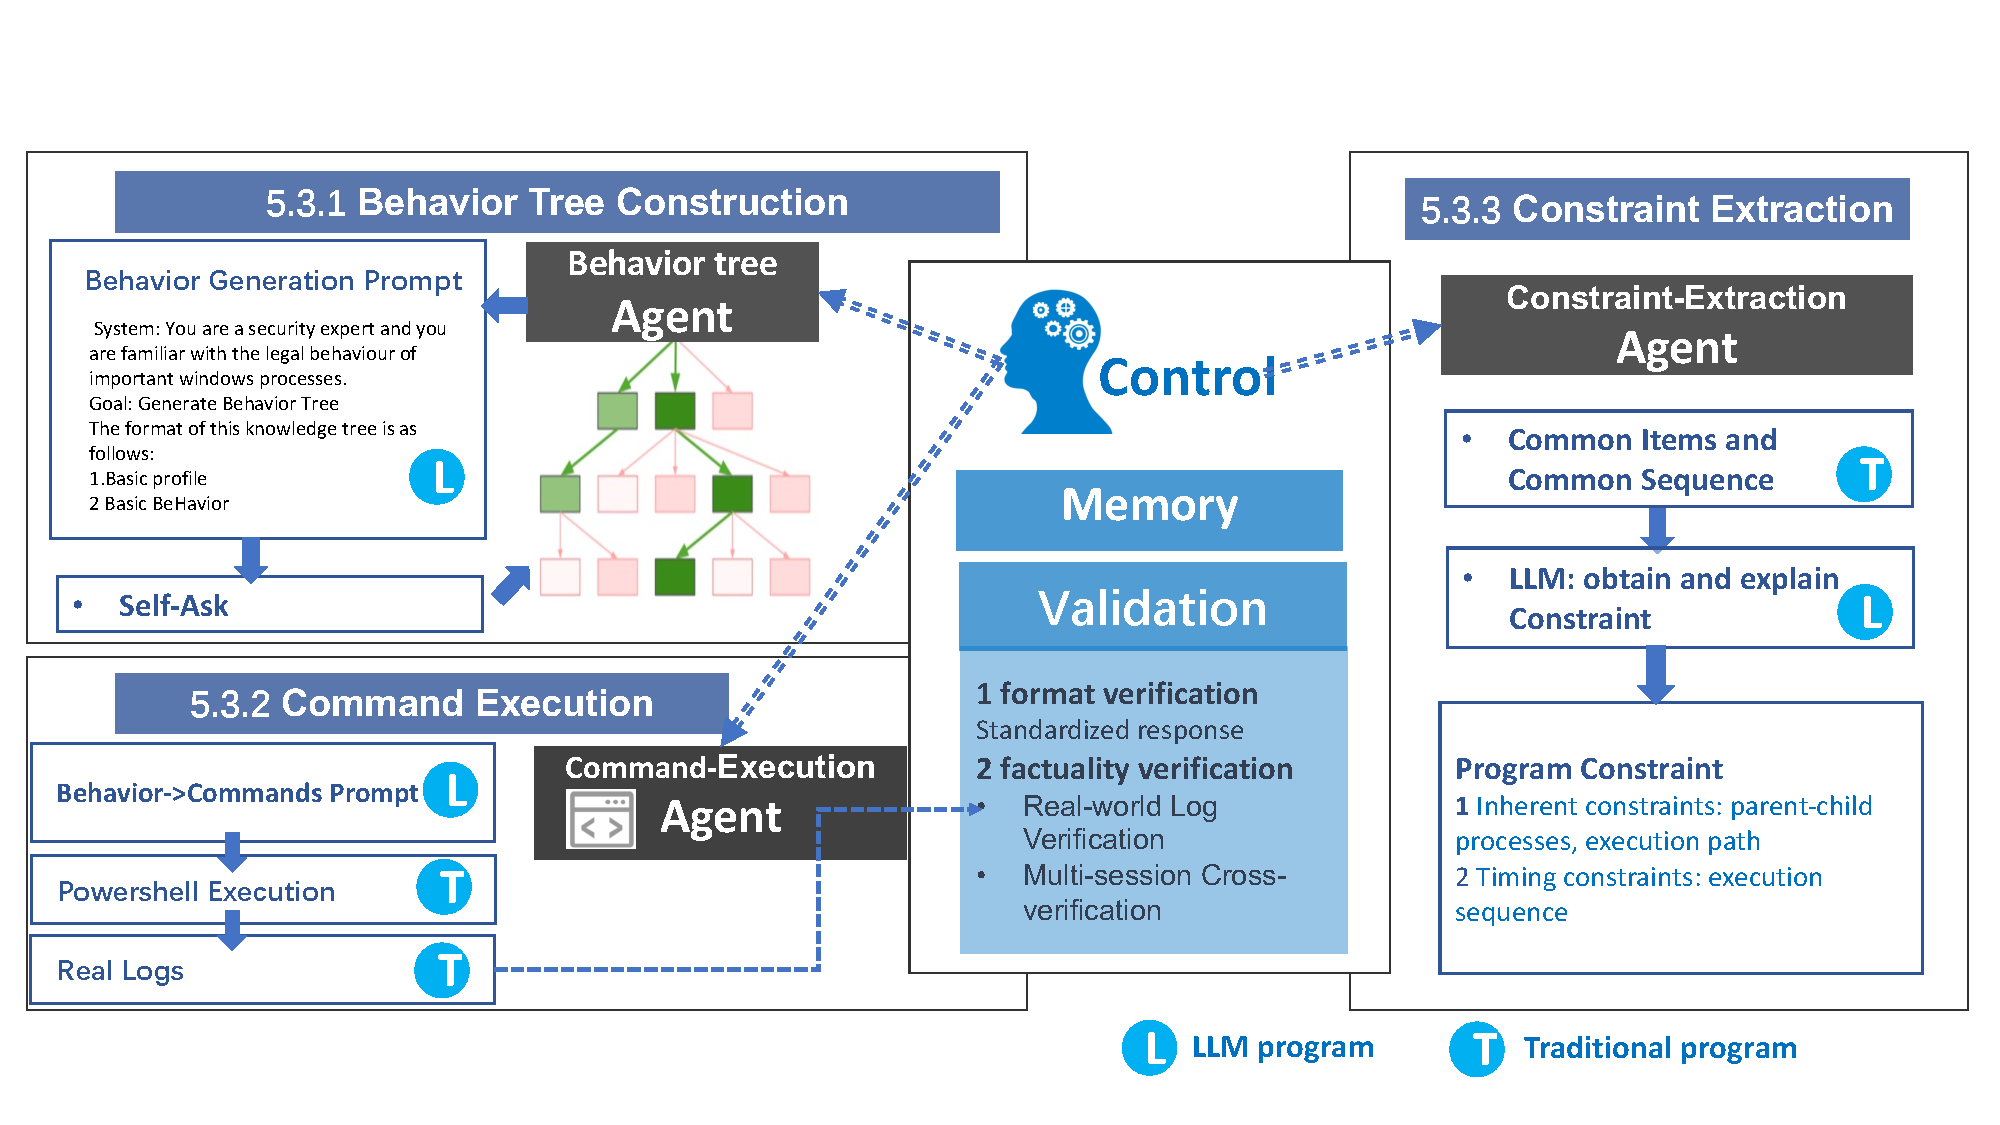
\includegraphics[width=0.48\textwidth]{figs/prompt.pdf}
%     \caption{The system is controlled by a central "controller" with memory storage and validation capabilities. The controller consists of three key modules: 1) Process Behavior Tree Construction Module, which maps out behavioral patterns; 2) Command Execution Module, which deploys active processes; and 3) Behavioral Invariants Extraction Module, which determines log-based requirements. These units meticulously craft program profiles using LLMs-assisted strategies and traditional methods.}
%     \label{fig-framework-prompt}
%     \end{figure}

\subsection{Definitions}\label{sec:toolDefs}

% \subsubsection{System Entity and System Event}
\noindent
{\bf System Entity.} In this work, we distinguish five principal entity categories: \textit{Processes}, \textit{Files}, \textit{Registry}, \textit{Dynamic Link Libraries (DLLs)}, and \textit{Network Connections}, the latter typically denoted by sockets. System entities possess unique attributes: the attributes associated with \textit{process} entities might include their Process ID (pid) or their executable paths. 

\noindent
{\bf System Event.} In this work, a system event $e$ is given by a tuple $\langle src, dst, rel, time\rangle$, where $src$ designates the source entity, constrained to only process entities, $dst$ indicates the target or destination entity, $rel$ denotes their interaction nature (e.g., writing into a file), and $time$ specifies the timestamp of the event occurrence.
We also illustrated the temporal relationship between events as $\langle e_1 \to e_2 \to e_3 \rangle$, indicating that the events occur in a logical sequence. 

% \begin{tabular}{|c|c|}
% \hline
% \textbf{Operation} & \textbf{Abbreviation} \\
% \hline
% Execution Path & EP \\
% \hline
% Parent Process & PP \\
% \hline
% Child Process & CP \\
% \hline
% Read & Re \\
% \hline
% Write & Wr \\
% \hline
% Create & Cr \\
% \hline
% RegSetValue & RS \\
% \hline
% RegAddValue & RA \\
% \hline
% Connect & Co \\
% \hline
% Load & Lo \\
% \hline
% \end{tabular}


\noindent
{\bf Proposition Definition.}
A proposition is represented as a triplet $\langle src, operation, dst\rangle$, where:
\begin{itemize}
    \item $src$ and $dst$ represent entities.
    \item Entities can be: Process, Dll, Registry, File, IP:port.
    \item An operation is performed from the $src$ to the $dst$.
\end{itemize}

\noindent
{\bf Behavioral Invariant.} In this work, the behavioral invariant is defined as a conjunction of a set of propositions, and its syntax is defined as follows:
\begin{align*}
 & \mathcal{I}  ::= \ \phi \mid \phi \wedge \mathcal{I} \\
 & \phi  \ \ \in \ \{ P_{ep}(x,y), \ P_{pp}(x,y), \ P_{cp}(x,Y), \ P_{a}(x,y), \ P_{o}(x_1,x_2,\ldots)\} \\
\end{align*}
where $P_{ep}(x,y)$ (resp. $P_{pp}(x,y)$) indicates that the execution path (parent process) of process $x$ is $y$, $P_{cp}(x, Y)$ indicates that the child processes of $x$ must come from processes set $Y$, $P_{a}(x,y)$ denotes that the process $x$ must execute the action $y$ in the future, and the proposition $P_{o}(x_1,x_2,\ldots)$ requires that the processes must be executed in the sequential order of $x_1,x_2,\ldots$.

% \begin{align*}
% \mathcal{I} & ::= P_{ep}(x,y) \mid p \wedge \mathcal{I} \\
% P_2 &: PP(X) = \text{"services.exe"} \\
% P_3 &: CP(X) \lor CP_2(X), CP_1(X) = \text{"dllhost.exe"} \\
% P_4 &: \text{Load}(X) = \text{"advapi32.dll"} \\
% P_5 &: \text{Order}(P_{51}, P_{52}), P_{51} = \text{Load}(\text{"advapi32.dll"}) \\
% \end{align*}
% Execution Path (EP): This denotes the path where the file svchost.exe resides.
% Parent Process (PP): This denotes the parent process of the current process or file.
% Child Process (CP): This denotes any child processes created by the current process or file.
% Load (Ld): This denotes the files or dynamic libraries that are loaded.

For example, a behavior invariant $\mathcal{I}_e$ of \texttt{svchost.exe} can be represented by the conjunction of the following propositions set: 

\begin{center}
$ \left\{
\begin{array}{c}
P_{ep}(\texttt{svchost.exe}, \text{``C:/windows/system32/''}),\\
 P_{pp}(\texttt{svchost.exe}, \texttt{services.exe}),\\
 P_{a}(\texttt{svchost.exe}, \text{Load(\texttt{advapi32.dll})})
\end{array} \right\}$
\end{center}

% $\{P_{ep}(\texttt{svchost.exe}, \text{"C:/windows/system32/"}), P_{pp}(\texttt{svchost.exe}, \text{"services.exe"}), P_{pp}(\texttt{svchost.exe}, \text{"Load(\texttt{services.exe})"}) \}$
% \begin{align*}
% P_{ep}(\texttt{svchost.exe}, \text{"C:/windows/system32/"}) \\
% P_{ep}(\texttt{svchost.exe}, \text{"C:/windows/system32/"})
% P_2 &: PP(X) = \text{"services.exe"} \\
% P_3 &: CP(X) \lor CP_2(X), CP_1(X) = \text{"dllhost.exe"} \\
% P_4 &: \text{Load}(X) = \text{"advapi32.dll"} \\
% P_5 &: \text{Order}(P_{51}, P_{52}), P_{51} = \text{Load}(\text{"advapi32.dll"}) \\
% \end{align*}
% \begin{align*}
% P_1 \land P_2 \land P_3 \land P_4 \land P_5
% \end{align*}

% The behavior invariant of \texttt{svchost.exe} is represented by the set of propositions
% \[ \{ P_1, P_2, P_3, P_4, P_5 \} \]
which states that the execution path of \texttt{svchost.exe} should be \text{"C:/windows/system32/"}, with parent process 
as \texttt{services.exe}, and it will load \texttt{advapi32.dll} finally.



\subsection{Process Preprocessing}
\noindent
{\bf Noisy Events Reduction.} 
We need to gather logs from different processes in the system to monitor processes.
Due to the large amount of logs, it becomes necessary to trim the data down. 
When behavioral processes are omitted, the normal functioning of the processes is not affected. Integration of domain knowledge enhances our ability to reduce redundant events. For example, there are also actions that are universal to all processes, such as loading \textit{ntdll.dll}. We've streamlined these ubiquitous events for a more concise representation.

% \subsubsection{Process Classification}
% \label{sec:classifition}
\noindent
{\bf Process Classification.} \label{sec:classifition}
We created a prompt to query  LLMs that classified these processes into legitimate, illegitimate, and uncertain names (due to the LLMs database's incompleteness).
Due to name confusion, many illegitimate process names can be changed to legitimate process names for further evaluation.
For both the legitimate and confusion processes, we construct profiles according to the methods described in the following sections. An investigator should investigate further illegitimate or unclear categories since they may contain malware.

\subsection{Behavioral Reference Construction}
As mentioned before, we intend to decompose the behavioral reference construction module into three subtasks that can be effectively tackled by LLMs. In this section, we provide more details for each of them.
\label{sec:profile_con}
% Next, we present our profile building module in detail, which consists of three agent components.

% In order to conduct the factual validation, multiple LLMs sessions are debating each other, as well as real-life logs being validated.
% This central program controller controls three distinct agent modules: the Process Behavior Tree Construction Module, the Command Execution Module, and the Log Constraint Extraction Module. Each module manages LLMs sessions and context independently, ensuring both coherence and specialized expertise. It combines LLMs-driven processes (like behavior tree construction) with conventional computational tasks (like frequent sequence mining). A combination of traditional and LLMs-driven processes is used to create detailed process profiles under program controller guidance.

\subsubsection{Process Behavior Tree Construction}
The construction of \textit{Process Behavior Trees} is one of the most important steps in the process.
First, we define the \textit{Process Behavior Tree}.

\begin{figure}[h]
    \centering
      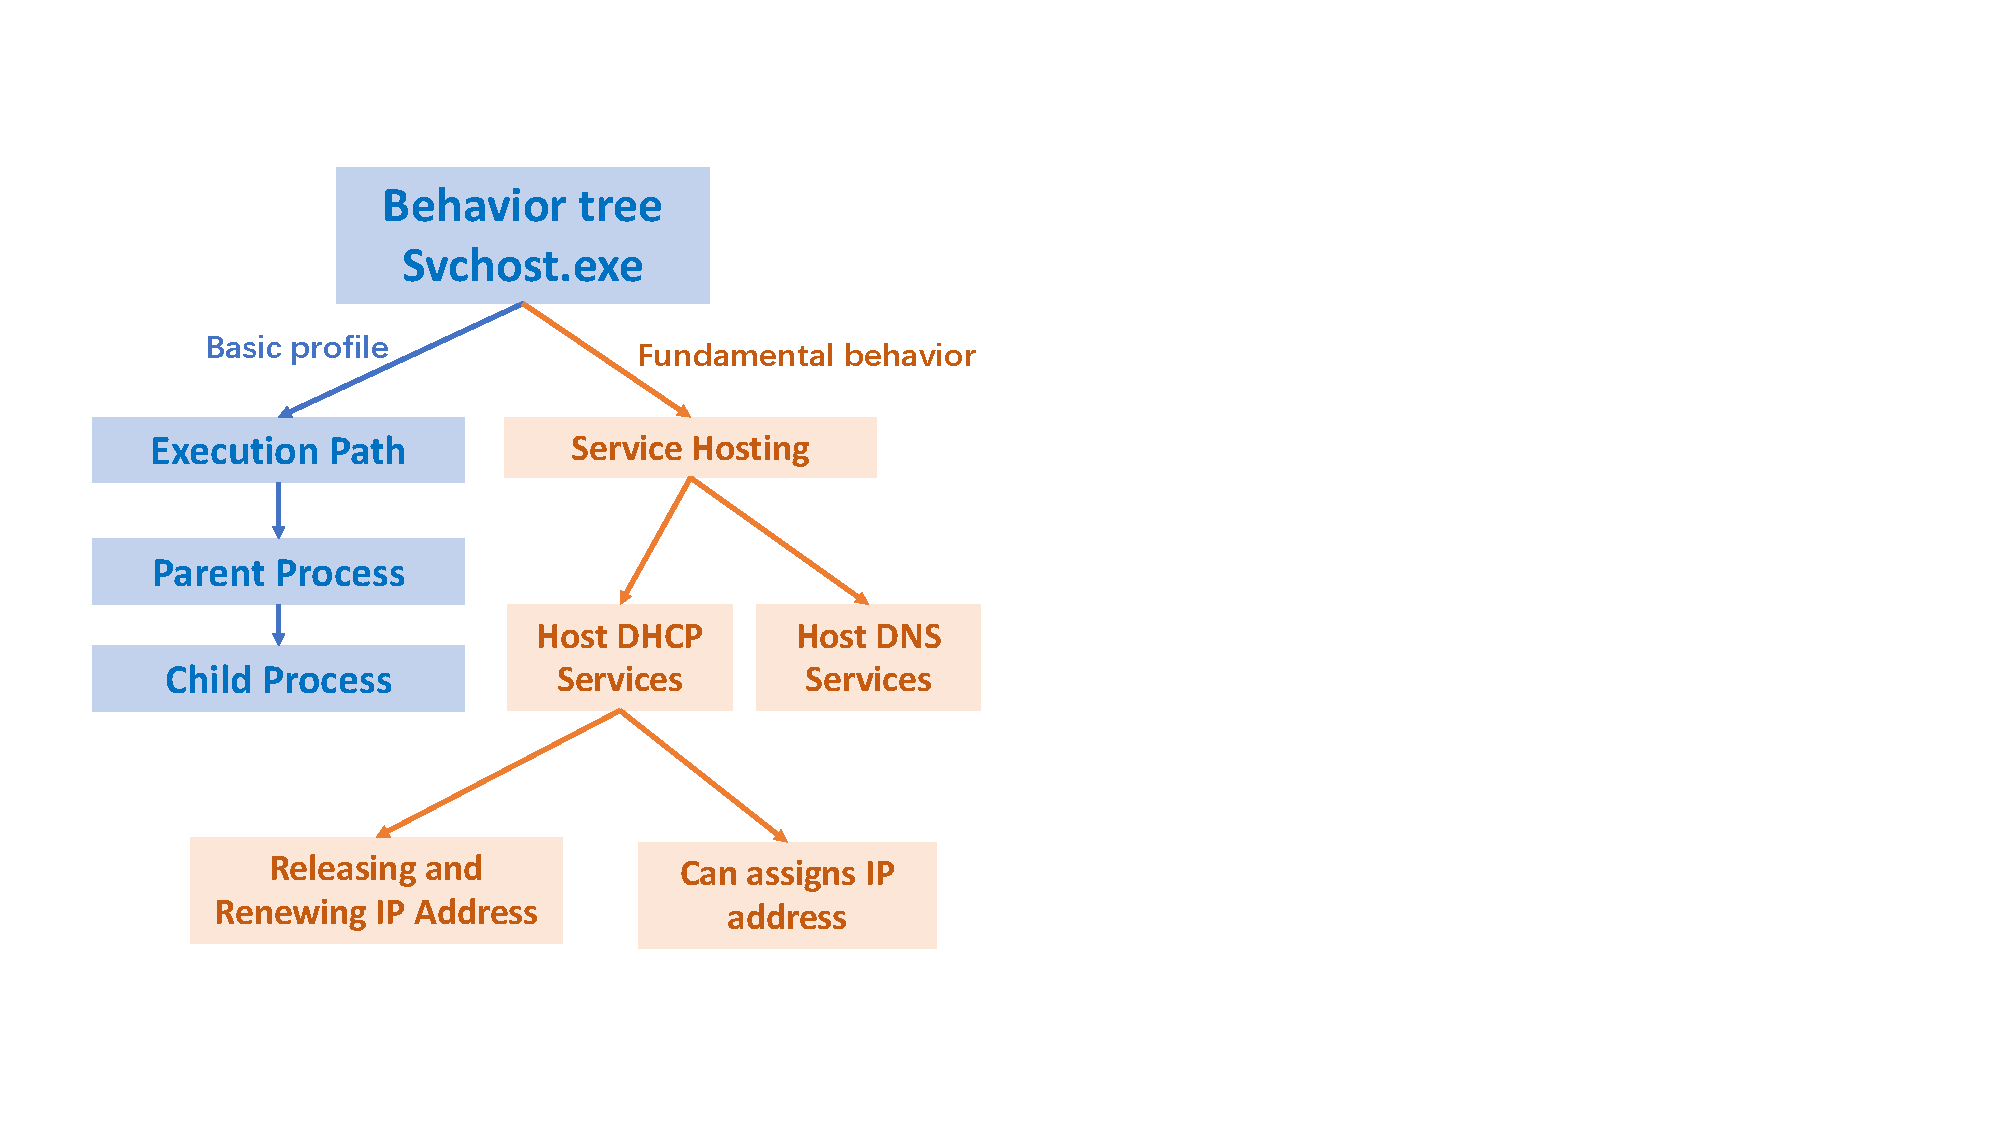
\includegraphics[width=0.35\textwidth]{figs/tree1.pdf}
    \caption{Process Behavior Tree Representation.}
    \label{fig:BT}
\end{figure}


% \begin{definition}[Process Behavior Tree]
% A Process Behavior Tree (BT) is a tuple \((N, B)\), where:
% \begin{enumerate}
%     \item \(N\) is a set of nodes organized in a tree structure. Each node represents legitimate behavior of a process. 
%     \item \(B\) is a function that assigns to each node \(n \in N\) a set of attributes \(B(n)\). Each attribute is a pair \((b, w)\), where \(b\) is the behavior name and \(w\) is a description or attribute of that behavior. 
% \end{enumerate}
% \end{definition}

To generate as many behaviors as possible, we've crafted two prompts: the \textit{Initialization Behavior Tree Prompt}(A detailed prompt can be found in the Appendix~\ref{prompt-init-tree}) and the \textit{Expansion Behavior Tree Prompt}. Initially, we employ the \textit{Initialization Behavior Tree Prompt} to create a foundational behavior tree. Subsequently, this tree is expanded through iterative rounds using the \textit{Expansion Behavior Tree Prompt}. In order to create a diversity and precision of behaviors, we have incorporated four strategies:

\noindent
{\bf Creating an Initial Process Behavior Tree:} To ensure a standardized behavior tree, we've defined a specific output format for the behavior tree.

\noindent
{\bf Updating Process Behavior Tree:}
The Behavior Tree Prompt uses self-ask techniques. The behavior tree can be expanded by allowing the LLMs to ask and answer its own questions.

\noindent
{\bf Using system role:} 
LLMs often ignore earlier details in a conversation, focusing on recent interactions. As a countermeasure, we leverage the benefits of the system role and embed both roles and objectives within it.

\noindent
{\bf Self-Evaluation:}
We aim to provide LLMs with the ability to self-criticize and review current nodes. If the LLMs determine that the branch does not require expansion, node expansion is stopped.

The resulting behavior tree is illustrated in Figure~\ref{fig:BT}. Taking the behavior tree of \textit{svchost.exe} as an example, we begin with the basic profile. This includes details such as the execution path of the process, its parent process (the parent process of \textit{svchost.exe} can only be \textit{services.exe}), and its child processes. Following this, we have the fundamental behaviors, such as service hosting, DLL loading, and service isolation exhibited by \textit{svchost.exe}. Focusing on the most significant behavior, which is service hosting, the behavior tree can be extended to detail the specific services being hosted. 

\subsubsection{Command Execution}

An initial step is to design a prompt (detailed prompts can be found in Appendix \ref{prompt-commands}) for generating commands from previous behavior trees. In order to obtain actual log files, this prompt generates corresponding system commands. We can validate some of the behaviors described in the previous step by collecting these logs. Using these logs, it is possible to directly verify some behaviors like parent processes, execution paths, and other details. It is, however, not possible to translate all system processes and behaviors into executable commands. In these cases, we employ the LLMs to produce relevant recommendations, which guide us in manually engaging with the system to obtain the required logs.

\subsubsection{Behavioral Invariants Extraction}\label{sec:BIE}

\begin{figure*}[h]
  \begin{subfigure}{.45\textwidth}
      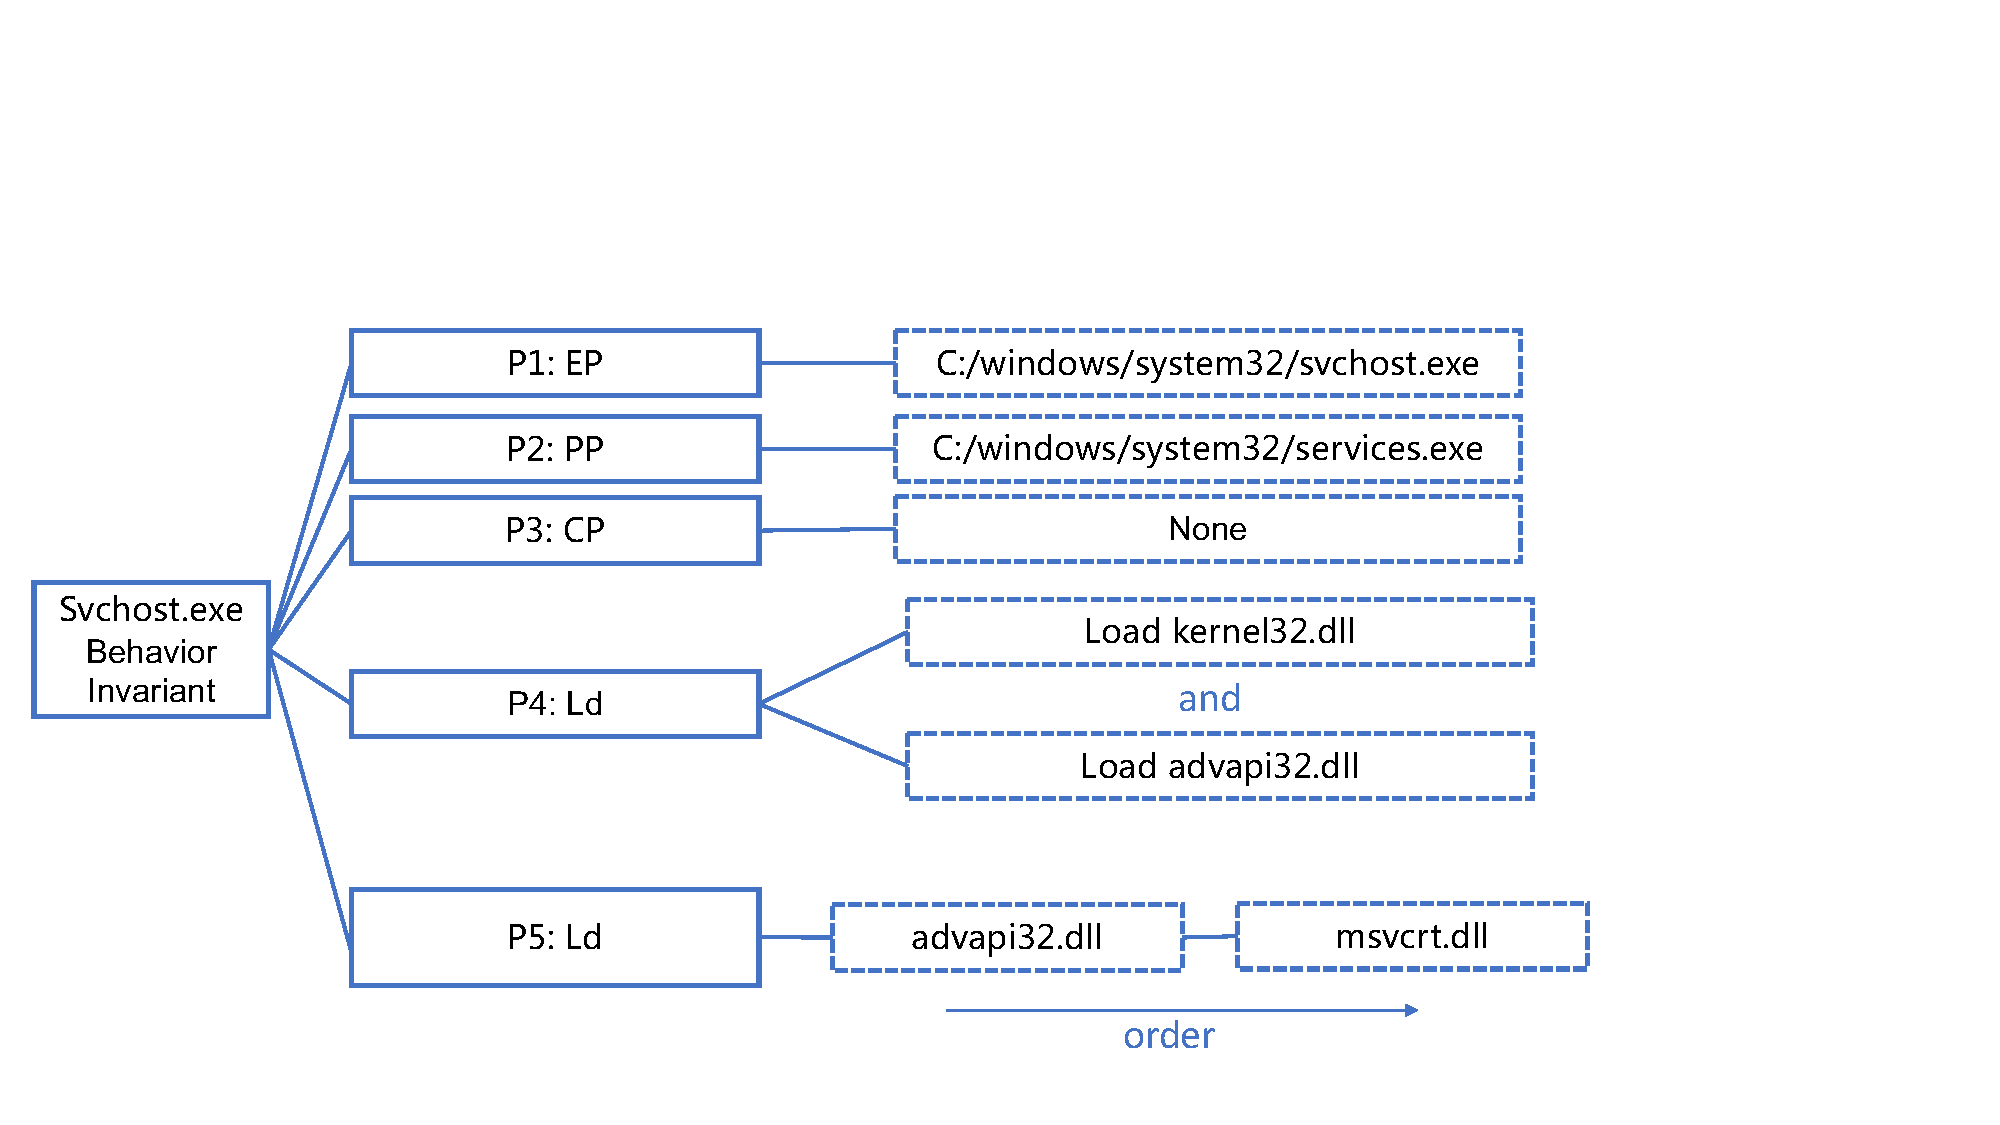
\includegraphics[width=\textwidth]{figs/cons-svchost.pdf}
      \caption{Behavioral Invariants of Svchost}
      \label{fig:cons-svchost}
  \end{subfigure}
  \hfill
  \begin{subfigure}{.5\textwidth}
      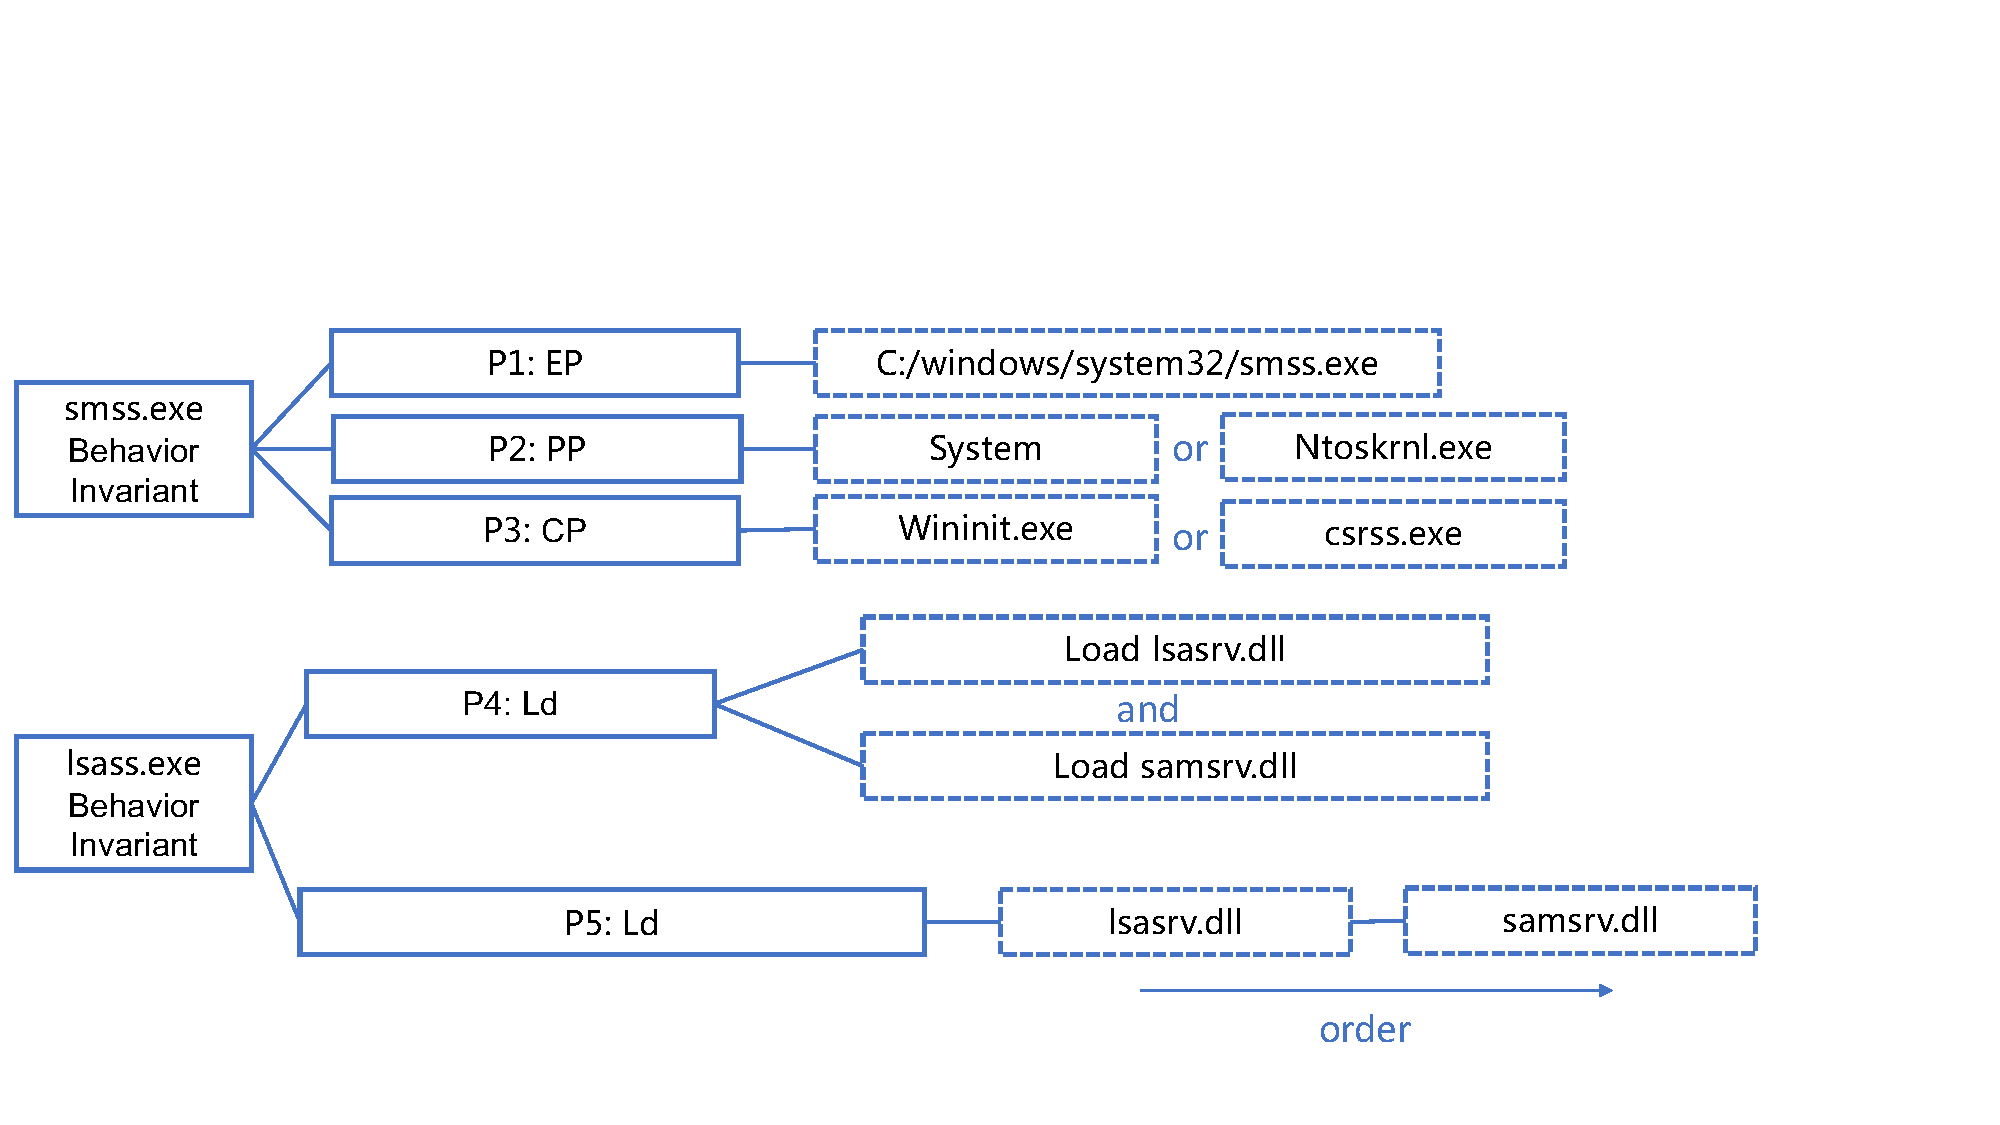
\includegraphics[width=\textwidth]{figs/cons-smss-lsass.pdf}
      \caption{Behavioral Invariants of Smss and Lsass}
      \label{fig:cons-smss-lsass}
  \end{subfigure}
  \hfill
  \caption{Behavioral Invariants}
  \label{fig:cons-def}
 \end{figure*}

The extraction of process behavioral invariants is a pivotal step in our methodology. We begin by categorizing behavioral invariants into five types as shown in Figure~\ref{fig:cons-def}.
The Figure~\ref{fig:cons-def} illustrates the behavioral invariants of three processes: \textit{svchost.exe}, \textit{lsass.exe}, and \textit{smss.exe}. In Figure~\ref{fig:cons-svchost}, the behavioral invariants of \textit{svchost.exe} are shown. There are five types of behavioral invariants: execution path, parent process, child process, intrinsic behavioral invariants (\textit{svchost.exe} will always load \textit{kernel32.dll} and \textit{advapi32.dll}.), and temporal behavioral invariants (\textit{advapi32.dll}, \textit{msvct.dll}, and \textit{kernelbase.dll} must be loaded in the specified sequence).
For certain processes, like \textit{smss.exe}, parent and child processes are optional. The parent process of \textit{smss.exe} can be \textit{system} or \textit{Ntoskml.exe}.

By comparing them with the logs gathered in the previous steps, we can validate and extract the first three behavioral invariants directly.
However, for intrinsic and temporal behavioral invariants, the challenge arises due to real-world logs' vastness. It is impractical to query the LLMs for each log due to memory constraints and its propensity to forget extended conversations. To overcome this, we designed a hybrid method that combines traditional programming techniques with queries to the LLMs to extract these two behavioral invariants.

We want to identify behaviors that are certain to occur in a specific process and in a certain order. 
We begin by mining the logs for common items among different log sequences.   
To speed up common sequence mining, we removed content from sequences that do not include common items when getting common items.
our next step is to use the PrefixSpan algorithm to find common sequences in these logs. 
To obtain the common sequences, rather than frequent sequences, we set the threshold \( \theta =1\) of the PrefixSpan algorithm, indicating that the sequence is certain to occur in the specified order.
(Algorithms are detailed in the Appendix~\ref{alg:fre-common}.
Having established the common items and sequences, we then direct our queries towards the LLMs, focusing specifically on these elements to extract intrinsic and temporal behavioral invariants. 
The detailed set of prompts used in this process is shown in Appendix~\ref{prompt-cons-explain}.


\paragraph{Explanation and Validation}
Furthermore, we request the LLMs to explain its findings, providing insights into these behavioral invariants.
Based on the prompt as shown in Appendix~\ref{prompt-cons-explain}, we ask LLMs to explain why this behavioral invariant exists, such as why \textit{lsass.exe} must load \textit{lsasrv.dll}, and why \textit{lsass.exe} must load \textit{samsrv.dll} after loading \textit{lsasrv.dll}. 
The LLMs would respond: \textit{lsass.exe} loads \textit{lsasrv.dll} primarily to utilize its code to complete tasks such as authentication and the generation of security tokens. 
\textit{lsass.exe} loads \textit{samsrv.dll} to manage and access the security account database, supporting user authentication and the implementation of local security policies

In addition, due to the potential for hallucinations or misleading results, it is imperative to ensure the accuracy and consistency of LLMs outputs. Due to this challenge, we developed a two-dimensional validation system.
\begin{itemize}
    \item Real-world Cross-referencing: LLMs outputs are executed as real-world commands, and their results are cross-checked against real-world logs.
    \item LLMs Multi-session Debates: The LLMs engage in iterative debates in multiple instances. Their goal is to find a consensus on an answer that is both accurate and reliable by verifying each other's responses and reasoning. They cannot reach a consensus on actions that are not entirely correct by having multiple LLMs debate each other. For definitive behaviors, they can eventually come to an agreement. A more detailed description of our approach can be found in the Appendix~\ref{prompt-cross-validation}.
\end{itemize}

\subsection{Runtime Behavioral Validation}
During this procedure, we extract propositions for both behavioral invariants deduced from the Behavioral Reference Construction module and original runtime system logs.

For behavioral invariants, characterized by their conjunctive composition of multiple propositions, we employ a direct extraction way to get the reference logical propositions set. For the runtime system logs, we adopt a method analogous to the one introduced in the ``Behavioral Invariants Extraction'' subtask from Section~\ref{sec:BIE}. In this manner, we construct a set of behavioral invariants from the original runtime system logs and then extract all propositions in these invariants as our runtime logical propositions. Finally, the consistency checking can be conducted between the two sets of propositions, and any inconsistency indicates a potential malicious attack.

